% Beamer presentation
\documentclass[11pt,aspectratio=43,ignorenonframetext,t]{beamer}

% Presentation settings
\mode<presentation>{
  \usetheme[framenumber,titleframestart=1]{UoM_alex}
  \usefonttheme{professionalfonts} % using non standard fonts for beamer
  \usefonttheme{serif}
  \usepackage{fontspec}
  \setmainfont[Ligatures=TeX]{Arial}
}

% Handout settings
\mode<article>{
  \usepackage{fullpage}
  \usepackage{fontspec}
  \setmainfont[Ligatures=TeX]{Arial}
  \setlength{\parskip}{1.5\baselineskip} % correct beamer line spacings
  \setlength{\parindent}{0cm}
  \usepackage{enumitem}
  \setlist[itemize]{topsep=0pt}
}

 % Packages
\usepackage{graphicx}
\graphicspath{{./images/png}} % generic graphics path; overridden if necessary
\usepackage{amsmath}
\allowdisplaybreaks[1] % allow eqnarrays to break across pages
\usepackage{amssymb} 
\usepackage[HTML]{xcolor}
\definecolor{uomlinkblue}{HTML}{0071BC}
\usepackage{hyperref}
\hypersetup{
  colorlinks=true,
  linkcolor=uomlinkblue,
  filecolor=uomlinkblue,      
  urlcolor=uomlinkblue,
  pdflang={en-GB},
}
\usepackage[document]{ragged2e} % left aligned text for accessibility
\usepackage{tikz}
\usetikzlibrary{positioning, arrows, arrows.meta}
\usepackage{unicode-math} % unicode maths for accessibility
\usepackage{pdfcomment}   % for alt text for accessibility
\usepackage{rotating}     % allow portrait figures and tables
\usepackage{subfigure}    % allow matrices of figures
\usepackage{float}        % allows H option on floats to force here placement
\usepackage{multirow}     % allows merging of rows in tables
\usepackage{tabularx}     % allows fixed width tables
\usepackage{ctable}       % modifies \hline for use in table
\usepackage{bm}           % allow bold fonts in equations
\usepackage{pgf}          % allow graphics manipulation
\usepackage{etoolbox}
  
% Custom commands
\newcolumntype{Z}{>{\centering\arraybackslash}X}  % tabularx centered columns 

\makeatletter
  \DeclareRobustCommand{\em}
  {
    \@nomath\em
    \if b
      \expandafter\@car\f@series\@nil \normalfont
    \else
      \bfseries
    \fi
  }
\makeatother

\makeatletter
  \preto{\@verbatim}{\topsep=0pt \partopsep=0pt}
\makeatother

\def\checkmark{
  \tikz\fill[scale=0.4](0,.35) -- (.25,0) -- (1,.7) -- (.25,.15) -- cycle;
}

% Counters
\newcounter{example_number} % keep track of the example questions

% Frontmatter
\newcommand{\cmclecture}[1]{
  \title{Combinatorial Mesh Calculus (CMC): Lecture #1}
}
\author{
  Lectured by:
  \href{https://scholar.google.com/citations?user=x4R-snQAAAAJ&hl=en}
  {Dr. Kiprian Berbatov}$^1$\\
  \smallskip
  Lecture Notes Compiled by:
  \href{https://scholar.google.com/citations?user=CoIpITkAAAAJ&hl=en}
  {Muhammad Azeem}$^1$\\
  \smallskip
  Under the supervision of:
  \href{https://scholar.google.co.uk/citations?user=3nWJe5wAAAAJ&hl=en}
  {Prof. Andrey P. Jivkov}$^1$\\
  \smallskip
  {\tiny $^1$Department of Mechanical and Aerospace Engineering,
    The University of Manchester, Oxford Road, Manchester M13 9PL, UK}
}

% Special frames
\newcommand{\cmctitleframe}{
  \titlepage
  \begin{tikzpicture}[remember picture,overlay]
    \node[anchor=south east] at (current page.south east) {
      \href{https://youtube.com/@kipi.berbatov}{
        
\includegraphics[width=1.5cm]{youtube-icon.png}
      }
    };
  \end{tikzpicture}
}
\newcommand{\cmcendframe}{
  \begin{figure}
    \centering
    
\includegraphics[width=0.85\linewidth]{Thanks.png}
  \end{figure}
}

\cmclecture{10}
\date{29 October 2025}

\begin{document}

%========================= TITLE =========================
\begin{frame}
  \cmctitleframe
\end{frame}


\begin{frame}{Diffeomorphisms}
\vspace{-0.2cm}
\begin{block}{Definition}
Let $n\in\mathbb{N}$ and $U,V\subseteq\mathbb{R}^n$. We say that $U$ and $V$ are \textbf{diffeomorphic} if there exist smooth maps
\[
f:U\to V, \quad g:V\to U
\]
such that $g\circ f=\operatorname{id}_U$ and $f\circ g=\operatorname{id}_V$. We write $U\cong V.$
\end{block}
\vspace{-0.2cm}
\begin{exampleblock}{Examples}
\begin{enumerate}
\item[1] $U=(-\frac{\pi}{2},\frac{\pi}{2})$, $V=\mathbb{R}$,
$f=\tan$, $g=\arctan$; both smooth.
\item[2] Any open $n$-brick $(a_1,b_1)\times\cdots\times(a_n,b_n)$ is diffeomorphic to $\mathbb{R}^n$.
\end{enumerate}
\end{exampleblock}
\end{frame}

\begin{frame}{Diffeomorphisms - Examples}
\begin{exampleblock}{Examples}
\begin{enumerate}
\item[3] $U=[0,\frac{\pi}{2})$, $V=\mathbb{R}_{\ge0}$, $\tan:U\to V$ is a diffeomorphism.
\item[4] Generalization: $U=[a_1,b_1)\times(a_2,b_2)\times\cdots\times(a_n,b_n)$,
$V=[0,\infty)\times\mathbb{R}^{n-1}$ are diffeomorphic by $\tan$–like component maps.
\end{enumerate}
\end{exampleblock}

\begin{center}
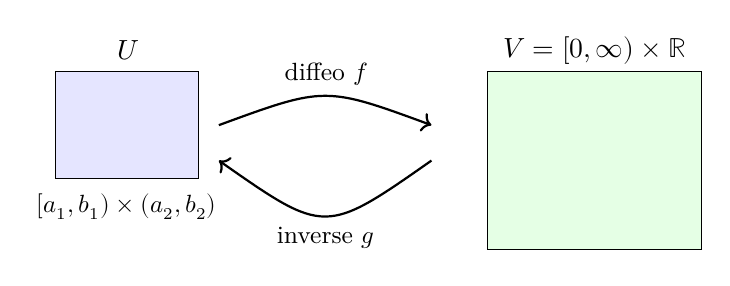
\begin{tikzpicture}[scale=0.9]
% Domain U
\begin{scope}[xshift=-3.8cm]
\draw[thick] (0,0) rectangle (2,1.5);
\node at (1,1.8) {$U$};
\fill[blue!10] (0,0) rectangle (2,1.5);
\node at (1,-0.4) {\small $[a_1,b_1)\times(a_2,b_2)$};
\end{scope}

% Codomain V
\begin{scope}[xshift=3.8cm]
\draw[thick] (-1.5,-1) rectangle (1.5,1.5);
\fill[green!10] (-1.5,-1) rectangle (1.5,1.5);
\node at (0,1.8) {$V=[0,\infty)\times\mathbb{R}$};
\end{scope}

% Mapping arrows
\draw[->, thick] (-1.5,0.75) .. controls (0,1.3) .. (1.5,0.75)
node[midway, above] {\small diffeo $f$};
\draw[->, thick] (1.5,0.25) .. controls (0,-0.8) .. (-1.5,0.25)
node[midway, below] {\small inverse $g$};
\end{tikzpicture}
\end{center}
\end{frame}

% --------------------------------------------------------------------
\begin{frame}{Smooth Manifolds (with Boundary)}
\begin{block}{Definition}
Let $m,n\in\mathbb{N}$ and $M\subseteq\mathbb{R}^{m+n}$.
We say that $M$ is a \textbf{smooth $n$–manifold (with boundary)} if for every $x\in M$ one of the following holds:
\begin{enumerate}
\item (\textit{Interior point})
There exists an open neighbourhood $V$ of $x$ ($x\in V\subseteq M$) in $M$ and an open set $U\subseteq\mathbb{R}^n$ together with a bijective immersion
$f:U\to V$ such that $Df$ has full rank $n$.
\item (\textit{Boundary point})
There exists a neighbourhood $V$ of $x$ ($x\in V\subseteq M$) in $M$ and $U\subseteq\mathbb{R}^n$ diffeomorphic to a half–space,
and a bijective immersion $f:U\to V$.
\end{enumerate}
\end{block}
\end{frame}


% --------------------------------------------------------------------
\begin{frame}{Examples of Manifolds}
\begin{exampleblock}{Examples}
\begin{enumerate}
\item Any open set $M\subseteq\mathbb{R}^n$ is a smooth $n$–manifold without boundary. For any $x\in M$ take $U=V=M$\ $f=\mathrm{id}_M$.
\item $n=2$, $M=\overline{B_1(0)}=\{(x,y)\in\mathbb{R}^2\mid x^2+y^2\le1\}$
is a 2–manifold with boundary $S^1=\{(x,y)\mid x^2+y^2=1\}$.
\item For $p=(1,0)\in S^1$, a chart can be built from a rectangle in parameter space mapping smoothly to a circular neighbourhood on $M$.
\end{enumerate}
\end{exampleblock}

\begin{center}
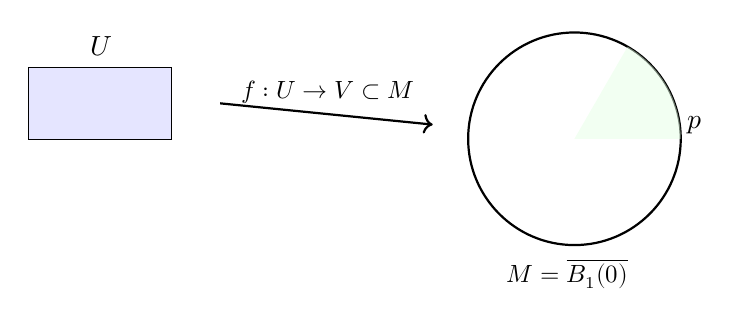
\begin{tikzpicture}[scale=0.9]
% Parameter space (U)
\begin{scope}[xshift=-4.2cm]
\draw[thick] (0,0) rectangle (2,1);
\node at (1,1.3) {$U$};
\fill[blue!10] (0,0) rectangle (2,1);
\end{scope}

% Circle M with chart image
\begin{scope}[xshift=3.5cm]
\draw[thick] (0,0) circle (1.5);
\fill[green!10, opacity=0.5] (1.5,0) arc (0:60:1.5) -- (0,0) -- cycle;
\node at (1.7,0.2) {$p$};
\node at (-0.1,-1.9) {\small $M=\overline{B_1(0)}$};
\end{scope}

% Arrow between them
\draw[->, thick] (-1.5,0.5) -- (1.5,0.2)
node[midway, above] {\small $f:U\to V\subset M$};
\end{tikzpicture}
\end{center}
\end{frame}


% --------------------------------------------------------------------
\begin{frame}{More Examples and Remarks}
\begin{exampleblock}{Examples}
\begin{enumerate}
\item[4] For any $n\in\mathbb{N}$,
\[
B_1(0)=\{(x_1,\dots,x_n)\in\mathbb{R}^n\mid x_1^2+\cdots+x_n^2<1\}
\]
is a smooth $n$–manifold with boundary $S^{n-1}$.
\item[5] The $(n-1)$–sphere
\[
S^{n-1}=\{(x_1,\dots,x_n)\in\mathbb{R}^n\mid x_1^2+\cdots+x_n^2=1\}
\]
is a smooth $(n-1)$–manifold without boundary.
\item[6] If $M$ is a smooth $n$–manifold with boundary $\partial M$, then
$\partial M$ is a smooth $(n-1)$–manifold without boundary and $\partial(\partial M)=\varnothing$.
\end{enumerate}
\end{exampleblock}
\end{frame}



\begin{frame}{Local Chart on the Circle near \(p=(1,0)\)}
\begin{block}{Note (efficient construction of a chart on \(S^1\))}
Let \(M=S^1=\{(x,y)\in\mathbb{R}^2\mid x^2+y^2=1\}\) and fix \(p=(1,0)\in S^1\).
Choose angles \(\alpha,\beta>0\) with \(\alpha+\beta<2\pi\), and set
\[
U:=(-\alpha,\beta)\subset\mathbb{R},\qquad
V:=\{(\cos\phi,\sin\phi)\mid \phi\in(-\alpha,\beta)\}\subset S^1.
\]
Define the map
\[
f:U\to V,\qquad f(\phi)=(\cos\phi,\sin\phi).
\]
Then \(f\) is a bijective immersion: its Jacobian (column) is
\[
Df(\phi)=
\begin{pmatrix}
-\sin\phi\\[2pt]
\phantom{-}\cos\phi
\end{pmatrix}\neq \begin{pmatrix}
0\\[2pt]
0
\end{pmatrix}\quad\text{for all }\phi\in U.
\]
\end{block}
\end{frame}

\begin{frame}{Local Chart on the Circle near \(p=(1,0)\)}
\begin{block}{Construction of a chart on \(S^1\))}
Hence \((U,f)\) is a smooth chart around \(p=f(0)\).
\emph{Why \(V\) cannot be all of \(S^1\):} the angle \(\phi\) is \(2\pi\)-periodic, so no single global parametrization \(\phi\mapsto (\cos\phi,\sin\phi)\) is injective on all of \(S^1\). One needs at least two overlapping charts (e.g.\ remove \((\pm1,0)\)) to cover \(S^1\).
\end{block}

\begin{center}
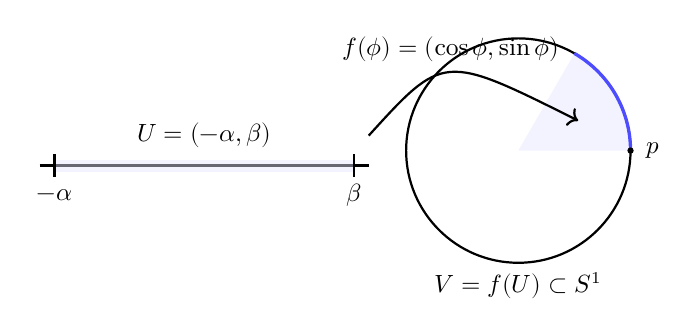
\begin{tikzpicture}[scale=0.95]
% circle S^1
\draw[thick] (0,0) circle (1.5);
% arc V
\fill[blue!10, opacity=0.45] (0,0)--(1.5,0) arc (0:60:1.5)--cycle;
\draw[blue!70, very thick] (1.5,0) arc (0:60:1.5);
% point p
\fill (1.5,0) circle (1.2pt); \node at (1.8,0) {\small \(p\)};
% labels
\node at (0,-1.8) {\small \(V=f(U)\subset S^1\)};
% domain interval U (schematic)
\begin{scope}[xshift=-4.2cm,yshift=-0.2cm]
\draw[thick] (-2.2,0) -- (2.2,0);
\fill[blue!10, opacity=0.45] (-2,0.08) rectangle (2,-0.08);
\draw[thick] (-2,0.15) -- (-2,-0.15); \node at (-2,-0.4) {\small \(-\alpha\)};
\draw[thick] ( 2,0.15) -- ( 2,-0.15); \node at ( 2,-0.4) {\small \(\beta\)};
\node at (0,0.4) {\small \(U=(-\alpha,\beta)\)};
\end{scope}
% arrow U -> V
\draw[->, thick] (-2.0,0.2) .. controls (-1.0,1.3) .. (0.8,0.4) node[midway, above] {\small \(f(\phi)=(\cos\phi,\sin\phi)\)};
\end{tikzpicture}
\end{center}
\end{frame}


\begin{frame}{Local Charts on a Smooth Manifold}
\begin{block}{Definition}
Let $M$ be a smooth $n$–manifold.
A \textbf{chart} (or local parametrization) on $M$ is a smooth bijective immersion
\[
f:U\to V,\quad U\subseteq_{\text{open}} M,
\]
where
\[
V\subseteq
\begin{cases}
\mathbb{R}^n, & \text{if } U\subseteq \operatorname{Int}(M),\\[2pt]
[0,\infty)\times\mathbb{R}^{n-1}, & \text{if } U\cap\partial M\neq\varnothing.
\end{cases}
\]
Both $f$ and its inverse $f^{-1}$ are smooth.
The components of $f$ define the \textit{local coordinates} on $U$.
\end{block}
\end{frame}

\begin{frame}{Local Charts on a Smooth Manifold}
\begin{block}{Intuition}
Each chart provides a smooth “flattening” of a curved region of $M$ into $\mathbb{R}^n$.
Locally, the manifold looks like ordinary Euclidean space, even if globally it may curve or close on itself.
\end{block}

\begin{center}
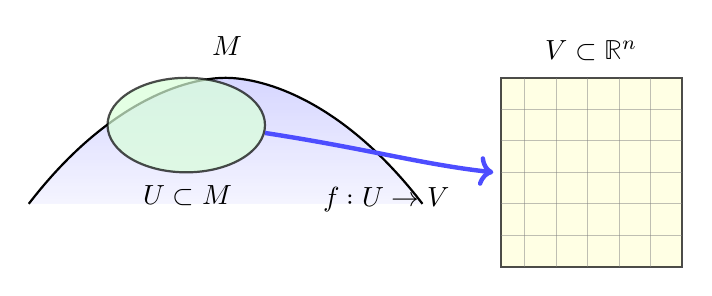
\begin{tikzpicture}[scale=1.0]
% Manifold patch with smoother shading
\shade[top color=blue!20, bottom color=blue!5, opacity=0.8]
    (-2.5,-1) .. controls (-1.5,0.3) and (-0.5,0.6) .. (0,0.6)
    .. controls (0.5,0.6) and (1.5,0.3) .. (2.5,-1) -- cycle;
\draw[thick] (-2.5,-1) .. controls (-1.5,0.3) and (-0.5,0.6) .. (0,0.6)
    .. controls (0.5,0.6) and (1.5,0.3) .. (2.5,-1);
\node at (0,1.0) {$M$};

% Chart domain with better positioning
\draw[thick, fill=green!15, opacity=0.7] (-0.5,0) ellipse (1.0 and 0.6);
\node at (-0.5,-0.9) {$U\subset M$};

% Plane patch with grid
\draw[thick, fill=yellow!15, opacity=0.7] (3.5,-1.8) rectangle (5.8,0.6);
\draw[gray, thin, opacity=0.5] (3.8,-1.8) -- (3.8,0.6);
\draw[gray, thin, opacity=0.5] (4.2,-1.8) -- (4.2,0.6);
\draw[gray, thin, opacity=0.5] (4.6,-1.8) -- (4.6,0.6);
\draw[gray, thin, opacity=0.5] (5.0,-1.8) -- (5.0,0.6);
\draw[gray, thin, opacity=0.5] (5.4,-1.8) -- (5.4,0.6);
\draw[gray, thin, opacity=0.5] (3.5,-1.4) -- (5.8,-1.4);
\draw[gray, thin, opacity=0.5] (3.5,-1.0) -- (5.8,-1.0);
\draw[gray, thin, opacity=0.5] (3.5,-0.6) -- (5.8,-0.6);
\draw[gray, thin, opacity=0.5] (3.5,-0.2) -- (5.8,-0.2);
\draw[gray, thin, opacity=0.5] (3.5,0.2) -- (5.8,0.2);
\node at (4.65,0.95) {$V\subset \mathbb{R}^n$};

% Mapping arrow with better curve
\draw[->, ultra thick, blue!70] (0.5,-0.1) .. controls (1.8,-0.3) and (2.5,-0.5) .. (3.4,-0.6);
\node at (2.0,-0.95) {$f:U\to V$};

\end{tikzpicture}
\end{center}
\end{frame}



\begin{frame}{Atlases and Transition Maps}
\begin{block}{Definition}
An \textbf{atlas} on a smooth manifold $M$ is a family of charts
\[
\{(U_i,f_i)\mid i\in I\},\quad \bigcup_{i\in I}U_i=M,
\]
such that all transition maps
\[
f_j\circ f_i^{-1}:f_i(U_i\cap U_j)\to f_j(U_i\cap U_j)
\]
are smooth wherever the charts overlap.
Different atlases that are compatible define the same smooth structure on $M$.
\end{block}

\end{frame}


\begin{frame}{Atlases and Transition Maps}
\begin{block}{Geometric Idea}
Each chart gives a local coordinate system, and their overlaps fit together smoothly.
This collection allows calculus on $M$.
\end{block}

\begin{center}
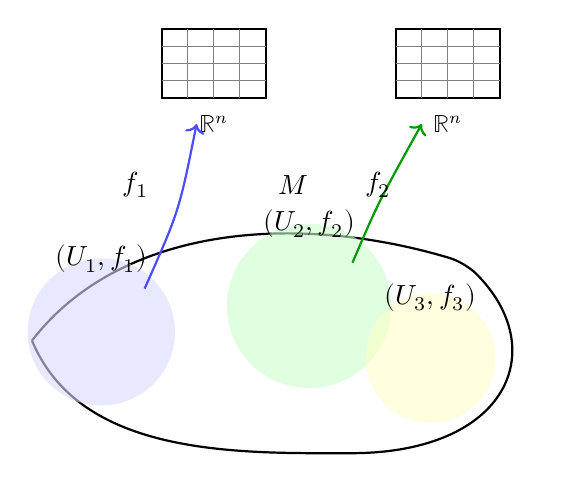
\begin{tikzpicture}[scale=1.1]
% Outline of manifold with smoother curve
\draw[thick, rounded corners=2mm] (-3,0) .. controls (-2,1.3) and (0,1.5) .. (2,0.9)
              .. controls (3,-0.1) and (2.5,-1.3) .. (0.5,-1.3)
              .. controls (-1,-1.3) and (-2.5,-1.2) .. (-3,0);
\node at (0,1.8) {$M$};

% Chart patches with better positioning
\fill[blue!15, opacity=0.6] (-2.2,0.1) circle (0.85);
\fill[green!20, opacity=0.6] (0.2,0.4) circle (0.95);
\fill[yellow!25, opacity=0.5] (1.6,-0.2) circle (0.75);

% Labels for charts
\node at (-2.2,0.95) {$(U_1,f_1)$};
\node at (0.2,1.35) {$(U_2,f_2)$};
\node at (1.6,0.5) {$(U_3,f_3)$};

% Coordinate planes
\begin{scope}[shift={(-1.5,2.8)}]
    \draw[thick] (0,0) -- (1.2,0) -- (1.2,0.8) -- (0,0.8) -- cycle;
    \draw[gray, thin] (0.3,0) -- (0.3,0.8);
    \draw[gray, thin] (0.6,0) -- (0.6,0.8);
    \draw[gray, thin] (0.9,0) -- (0.9,0.8);
    \draw[gray, thin] (0,0.2) -- (1.2,0.2);
    \draw[gray, thin] (0,0.4) -- (1.2,0.4);
    \draw[gray, thin] (0,0.6) -- (1.2,0.6);
    \node at (0.6,-0.3) {\small $\mathbb{R}^n$};
\end{scope}

\begin{scope}[shift={(1.2,2.8)}]
    \draw[thick] (0,0) -- (1.2,0) -- (1.2,0.8) -- (0,0.8) -- cycle;
    \draw[gray, thin] (0.3,0) -- (0.3,0.8);
    \draw[gray, thin] (0.6,0) -- (0.6,0.8);
    \draw[gray, thin] (0.9,0) -- (0.9,0.8);
    \draw[gray, thin] (0,0.2) -- (1.2,0.2);
    \draw[gray, thin] (0,0.4) -- (1.2,0.4);
    \draw[gray, thin] (0,0.6) -- (1.2,0.6);
    \node at (0.6,-0.3) {\small $\mathbb{R}^n$};
\end{scope}

% Arrows to coordinate planes
\draw[->, thick, blue!70] (-1.7,0.6) .. controls (-1.3,1.5) .. (-1.1,2.5);
\node at (-1.8,1.8) {$f_1$};

\draw[->, thick, green!60!black] (0.7,0.9) .. controls (1.0,1.6) .. (1.5,2.5);
\node at (1.0,1.8) {$f_2$};

\end{tikzpicture}
\end{center}
\end{frame}


\begin{frame}{Example}
\begin{block}{Construction}
Let \(M=S^1=\{(x,y)\in\mathbb{R}^2\mid x^2+y^2=1\}\).
Since \(f(\phi)=(\cos\phi,\sin\phi)\) is \(2\pi\)–periodic, no single chart covers all of \(S^1\).
We define two overlapping charts:
\[
\begin{aligned}
U_1 &= S^1\setminus\{(1,0)\}, & f_1(\phi)&=(\cos\phi,\sin\phi), & \phi\in(0,2\pi),\\[3pt]
U_2 &= S^1\setminus\{(-1,0)\}, & f_2(\theta)&=(\cos\theta,\sin\theta), & \theta\in(-\pi,\pi).
\end{aligned}
\]
On the overlap \(U_1\cap U_2\), the transition map \(f_2^{-1}\circ f_1\) is smooth,
hence $\{(U_1,f_1),(U_2,f_2)\}$ forms an atlas.
\end{block}

\end{frame}


\begin{frame}{Example}
\begin{center}
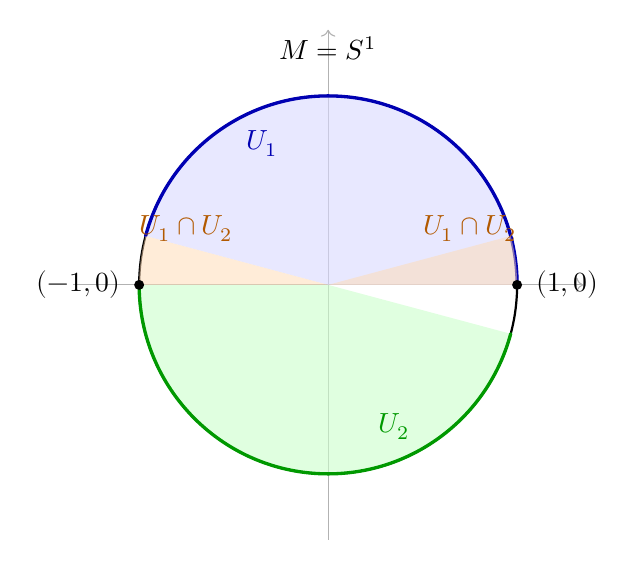
\begin{tikzpicture}[scale=1.2]
% Axes (drawn first, behind circle)
\draw[->, thin, gray!60] (-2.7,0)--(2.7,0);
\draw[->, thin, gray!60] (0,-2.7)--(0,2.7);

% Circle
\draw[thick, black] (0,0) circle (2);
\node at (0,2.5) {$M=S^1$};

% Chart 1 (blue arc) - slightly adjusted angle
\fill[blue!15, opacity=0.6] (0,0)--(2,0) arc (0:165:2)--cycle;
\draw[blue!70!black, very thick, line cap=round] (2,0) arc (0:165:2);
\node[blue!70!black] at (-0.7,1.5) {$U_1$};

% Chart 2 (green arc) - slightly adjusted angle
\fill[green!20, opacity=0.6] (0,0)--(-2,0) arc (180:345:2)--cycle;
\draw[green!60!black, very thick, line cap=round] (-2,0) arc (180:345:2);
\node[green!60!black] at (0.7,-1.5) {$U_2$};

% Overlap regions (both sides)
\fill[orange!30, opacity=0.5] (0,0)--(2,0) arc (0:15:2)--cycle;
\fill[orange!30, opacity=0.5] (0,0)--(-2,0) arc (180:165:2)--cycle;

% Overlap label
\node[orange!70!black] at (1.5,0.6) {$U_1\cap U_2$};
\node[orange!70!black] at (-1.5,0.6) {$U_1\cap U_2$};

% Points with better positioning
\fill[black] (2,0) circle (1.5pt);
\node[right] at (2.1,0) {$(1,0)$};
\fill[black] (-2,0) circle (1.5pt);
\node[left] at (-2.1,0) {$(-1,0)$};

\end{tikzpicture}
\end{center}
\end{frame}

\begin{frame}{Smooth Maps between Manifolds}
\vspace{-0.3cm}
\begin{block}{Definition}
Let $M,N$ be smooth manifolds with $\dim M=m$ and $\dim N=n$.
A map $f:M\to N$ is \textbf{smooth} if for every chart $(U,\phi)$ on $M$ and every chart $(V,\psi)$ on $N$ with $f(U)\subseteq V$,
the composition
\vspace{-0.1cm}
\[
\psi\circ f\circ\phi^{-1} : \phi(U)\subseteq\mathbb{R}^m \to \mathbb{R}^n
\]
is smooth in the classical sense.
The space of all smooth maps is denoted $C^{\infty}(M,N)$.
If $N=\mathbb{R}$, we write $\mathcal{F}(M):=C^{\infty}(M,\mathbb{R})$ — a commutative $\mathbb{R}$–algebra with unity.
\end{block}
\vspace{-0.3cm}
\begin{center}
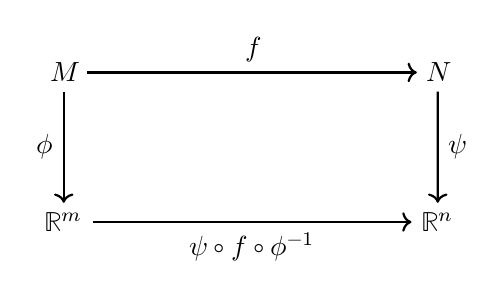
\begin{tikzpicture}[scale=0.95]
\node (M) at (0,0) {$M$};
\node (N) at (5,0) {$N$};
\node (Rm) at (0,-2) {$\mathbb{R}^m$};
\node (Rn) at (5,-2) {$\mathbb{R}^n$};

\draw[->, thick] (M)--(N) node[midway, above] {$f$};
\draw[->, thick] (M)--(Rm) node[midway, left] {$\phi$};
\draw[->, thick] (N)--(Rn) node[midway, right] {$\psi$};
\draw[->, thick] (Rm)--(Rn) node[midway, below] {$\psi\circ f\circ\phi^{-1}$};
\end{tikzpicture}
\end{center}
\end{frame}


% --------------------------------------------------------------------
\begin{frame}{Example: Inclusion $S^1\hookrightarrow S^2$}
\vspace{-0.2cm}
\begin{block}{Example}
Let
\vspace{-0.4cm}
\begin{align*}
    M=S^1=&\{(x,y)\in\mathbb{R}^2\mid x^2+y^2=1\},\\
N=S^2=&\{(x,y,z)\in\mathbb{R}^3\mid x^2+y^2+z^2=1\},
\end{align*}
and define $f:M\to N$ by $f(x,y)=(x,y,0)$. For charts:
\begin{align*}
\alpha:&(E,F)\to U,\quad \alpha(\phi)=(\cos\phi,\sin\phi),\\
\beta:&(A,B)\times(C,D)\to V,\quad \beta(\theta,\phi)=(\sin\theta\cos\phi,\sin\theta\sin\phi,\cos\theta).
\end{align*}
Then
\[
\beta\!\left(\frac{\pi}{2},\phi\right)=(\cos\phi,\sin\phi,0)=f(\cos\phi,\sin\phi)=f(\alpha(\phi)),
\]
showing the compatibility of local charts.
\end{block}
\end{frame}

\begin{frame}{Example}
\begin{center}
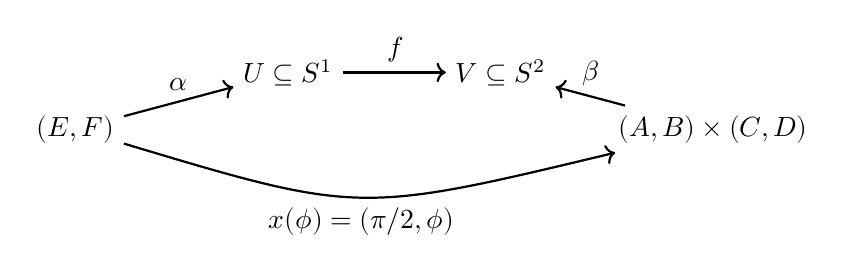
\begin{tikzpicture}[scale=0.9]
\node (E) at (0,0) {$(E,F)$};
\node (U) at (3,0.8) {$U\subseteq S^1$};
\node (V) at (6,0.8) {$V\subseteq S^2$};
\node (A) at (9,0) {$(A,B)\times(C,D)$};

\draw[->, thick] (E)--(U) node[midway, above] {$\alpha$};
\draw[->, thick] (U)--(V) node[midway, above] {$f$};
\draw[->, thick] (A)--(V) node[midway, above] {$\beta$};

\draw[->, thick] (E) .. controls (4,-1.2) .. (A) node[midway, below] {$x(\phi)=(\pi/2,\phi)$};
\end{tikzpicture}
\end{center}
\end{frame}


% --------------------------------------------------------------------
\begin{frame}{Vector Fields on a Smooth Manifold}
\begin{block}{Definition}
Let $M$ be a smooth manifold.
A \textbf{vector field} on $M$ is an operator $X:\mathcal{F}(M)\to\mathcal{F}(M)$ satisfying:
\begin{enumerate}
\item $\forall f,g\in\mathcal{F}(M)$, $X(fg)=X(f)g+fX(g)$ \hfill (Leibniz rule)
\item $X$ is $\mathbb{R}$–linear.
\end{enumerate}
\end{block}

\begin{exampleblock}{Examples}
\begin{itemize}
\item $M=\mathbb{R}$, $X=\dfrac{d}{dx}$, then $X(fg)=f'g+fg' (=\frac{\partial f}{\partial x}g + f\frac{\partial g}{\partial x})$.
\item $M=\mathbb{R}^n$, $X=\displaystyle\sum_{i=1}^{n} X^i(x)\dfrac{\partial}{\partial x_i}$.
\end{itemize}
\end{exampleblock}
\end{frame}


% --------------------------------------------------------------------
\begin{frame}{The Module of Vector Fields}
\vspace{-0.3cm}
\begin{block}{Theorem}
Let $M$ be a smooth manifold and $\mathcal{X}(M)$ the set of vector fields on $M$.
Define scalar multiplication by
\vspace{-0.2cm}
\[
(fX)(g)=f\,(Xg), \qquad f,g\in\mathcal{F}(M),\ X\in\mathcal{X}(M).
\]
Then $(\mathcal{X}(M),+,\cdot)$ is an $\mathcal{F}(M)$–module.
\end{block}
\vspace{-0.3cm}
\begin{block}{Local Form}
If $(U,\phi)$ is a chart with coordinates $(x_1,\dots,x_n)$, then
\vspace{-0.2cm}
\[
\mathcal{X}(U)\text{ is a free $\mathcal{F}(U)$–module with basis }
\frac{\partial}{\partial x_1},\dots,\frac{\partial}{\partial x_n}.
\]
Every $X\in\mathcal{X}(U)$ can be expressed as
\vspace{-0.2cm}
\[
X=f_1\frac{\partial}{\partial x_1}+\cdots+f_n\frac{\partial}{\partial x_n}, \quad f_i\in\mathcal{F}(U).
\]
\vspace{-0.5cm}
\end{block}
\end{frame}


% --------------------------------------------------------------------
\begin{frame}{Example: Euler Vector Field in $\mathbb{R}^2$}
\begin{block}{Example}
The \textbf{Euler vector field} on $\mathbb{R}^2$ is
\[
X = x\frac{\partial}{\partial x} + y\frac{\partial}{\partial y}.
\]
For $f(x,y)$, we have
\[
Xf = x\frac{\partial f}{\partial x} + y\frac{\partial f}{\partial y}.
\]
\end{block}
\end{frame}

\begin{frame}{Example: Euler Vector Field in $\mathbb{R}^2$}
\begin{block}{}
\begin{center}
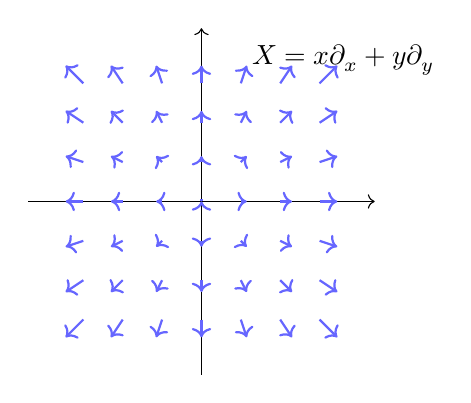
\begin{tikzpicture}[scale=1.0]
% Axes
\draw[->] (-2.2,0)--(2.2,0);
\draw[->] (0,-2.2)--(0,2.2);
% Vector field arrows
\foreach \x in {-1.5,-1,-0.5,0,0.5,1,1.5}{
\foreach \y in {-1.5,-1,-0.5,0,0.5,1,1.5}{
\draw[->, thick, blue!60] (\x,\y)--(\x+0.15*\x,\y+0.15*\y);
}}
\node at (1.8,1.8) {$X=x\partial_x+y\partial_y$};
\end{tikzpicture}
\end{center}
\end{block}
\end{frame}

% --------------------------------------------------------------------
\begin{frame}{Differential Forms}
\begin{block}{Definition}
Let $M$ be a smooth manifold.
The space of differential forms is
\[
\Omega^{\bullet}(M) := \Lambda^{\bullet}((\mathcal{X}(M))^*).
\]
If $\dim M=n$, in local coordinates $(x_1,\dots,x_n)$,
the basis of $\mathcal{X}(U)$ is $\partial/\partial x_i$, and the dual basis of $(\mathcal{X}(U))^*=\Omega^1(U)$ is $dx_i$, satisfying
\[
dx_i\!\left(\frac{\partial}{\partial x_j}\right)=\delta_{ij}.
\]
\end{block}
\end{frame}

\begin{frame}{Differential Forms}
    \begin{exampleblock}{Examples}
\begin{itemize}
\item $\mathbb{R}^2$: $\Omega^0M=\mathcal{F}(M)$,\\
\begin{itemize}
\item $\Omega^1M=\{f_xdx+f_ydy\}$,\\
\item$\Omega^2M=\{g\,dx\wedge dy\}$.
\end{itemize}
\item $\mathbb{R}^3$:
\begin{itemize}
\item $\Omega^0M=\mathcal{F}(M)$,\\
\item $\Omega^1M=\{f_1dx+f_2dy+f_3dz\}$,\\
\item $\Omega^2M=\{g_1dy\wedge dz+g_2dz\wedge dx+g_3dx\wedge dy\}$,\\
\item $\Omega^3M=\{h\,dx\wedge dy\wedge dz\}$.
\end{itemize}
\end{itemize}
\end{exampleblock}
\end{frame}


% --------------------------------------------------------------------
\begin{frame}{Exterior Derivative}
\begin{block}{Definition}
For a smooth manifold $M$, the exterior derivative is the graded operator
\[
d:\Omega^{\bullet}(M)\to\Omega^{\bullet}(M),
\quad d_p:\Omega^p(M)\to\Omega^{p+1}(M),
\]
defined by:
\begin{enumerate}
\item For $f\in\Omega^0(M)=\mathcal{F}(M)$,
\[
df=\frac{\partial f}{\partial x_1}dx_1+\cdots+\frac{\partial f}{\partial x_n}dx_n.
\]
\item For $\omega,\eta\in\Omega^{\bullet}(M)$,
\[
d(\omega\wedge\eta)=d\omega\wedge\eta+(-1)^{\deg\omega}\omega\wedge d\eta.
\]
\end{enumerate}
\end{block}

\end{frame}

\begin{frame}{Exterior Derivative}
\begin{block}{Definition}
\begin{enumerate}
\item[3] $d_{p+1}\circ d_p=0$ (cochain complex property).
\end{enumerate}
\end{block}


\begin{center}
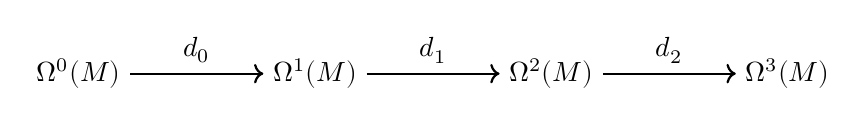
\begin{tikzpicture}[scale=1]
\node (F) at (0,0) {$\Omega^0(M)$};
\node (W1) at (3,0) {$\Omega^1(M)$};
\node (W2) at (6,0) {$\Omega^2(M)$};
\node (W3) at (9,0) {$\Omega^3(M)$};

\draw[->, thick] (F)--(W1) node[midway, above] {$d_0$};
\draw[->, thick] (W1)--(W2) node[midway, above] {$d_1$};
\draw[->, thick] (W2)--(W3) node[midway, above] {$d_2$};
\end{tikzpicture}
\end{center}
\end{frame}

% --------------------------------------------------------------------
\begin{frame}{Example: Gradient and Curl in $\mathbb{R}^2$}
\begin{block}{Example}
Let $M=\mathbb{R}^2$ and $f\in\Omega^0(M)$,
then
\[
df = \frac{\partial f}{\partial x}\,dx + \frac{\partial f}{\partial y}\,dy = (\nabla f)^{\flat}.
\]
For $\omega = P\,dx + Q\,dy \in \Omega^1(M)$,
\[
d\omega = \left(\frac{\partial Q}{\partial x} - \frac{\partial P}{\partial y}\right) dx\wedge dy,
\]
which corresponds to the curl of $(P,Q)$.
\end{block}

\end{frame}

\begin{frame}{Example: Gradient and Curl in $\mathbb{R}^2$}
\begin{block}{Example}
\begin{center}
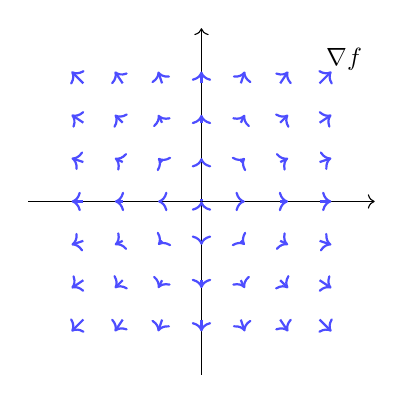
\begin{tikzpicture}[scale=1]
% Axes
\draw[->] (-2.2,0)--(2.2,0);
\draw[->] (0,-2.2)--(0,2.2);
% Gradient arrows
\foreach \x in {-1.5,-1,-0.5,0,0.5,1,1.5}{
\foreach \y in {-1.5,-1,-0.5,0,0.5,1,1.5}{
\draw[->, thick, blue!70] (\x,\y)--(\x+0.1*\x,\y+0.1*\y);
}}
\node at (1.8,1.8) {\small $\nabla f$};
\end{tikzpicture}
\end{center}
\end{block}
\end{frame}




% --------------------------------------------------------------------
\begin{frame}{Summary of Lecture}
\vspace{-0.3cm}
\begin{itemize}
\item Introduced diffeomorphisms and smooth manifolds.
\item Described examples: disks, spheres, and general $n$–bricks as manifolds or manifolds with corners.
\item Defined charts, local coordinates, and atlases with geometric illustrations.
\item Demonstrated circle parametrization and Jacobian regularity for immersion.
\item Defined smooth maps between manifolds using charts and commutative diagrams.
\item Introduced vector fields as derivations and showed $\mathcal{X}(M)$ is an $\mathcal{F}(M)$–module. Illustrated the Euler vector field on $\mathbb{R}^2$ geometrically.
\item Defined differential forms, and exterior derivative. Showed $d_{p+1}\circ d_p=0$, relating gradients and curls in $\mathbb{R}^2$ to Green’s theorem.
\end{itemize}
\end{frame}

\begin{frame}{Thanks}
  \cmcendframe
\end{frame}

\end{document}
